\articlehead{Carroll Ballad's Duma}{JM}{2013}

\textit{Duma} (2005) is Carroll Ballard's fourth and final great animal film. I've discussed \textit{The Black Stallion} (1979) and \textit{Fly Away Home} (1996) before; I'll eventually round out my series with \textit{Never Cry Wolf} (1983).

\textit{Duma} is the name of a cheetah, one of the protagonists in the film. He and Xan, a young boy, take a journey through southern Africa.

\begin{figure}
  \begin{center}
    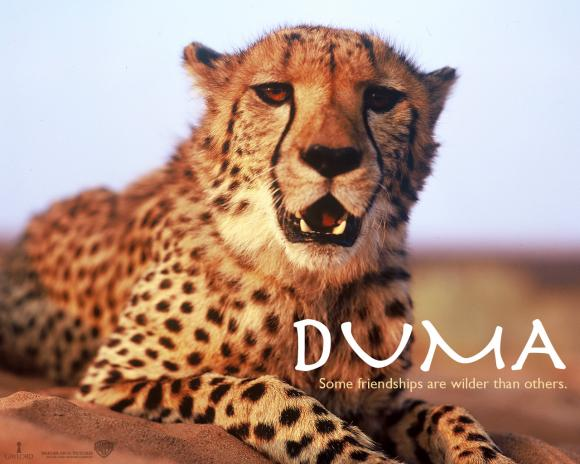
\includegraphics[width=\textwidth]{content/assets/duma--1}
  \end{center}
  \caption{Cheetahs: thinking skills need work}
\end{figure}

I want to start this article by talking about \textit{Duma}, and what I learned about cheetahs from watching this film. I learned that cheetahs are morons.

There are plenty of cat antics in the film. But Duma is no lolcat. He is docile, obedient, and permanently confused/apathetic. He has a blank-faced stare that betrays a lack of understanding, and a lack of curiosity. If you put Duma on a giant roomba, he'd just sit down and look bewildered.

It's a running joke in the film that Duma is part domesticated, so his survival skills are hopeless. His hunting in particular is portrayed as being somewhere around the ``I can't find my food bowl'' level. At one point, he saves the day ``hunting'': he lopes after an ostrich and eventually stumbles/gets confused by a nest full of eggs. Success through incompetence.

So you might think that \textit{Duma}'s boneheadedness is a deliberate plot device, and that he's merely the Sarah Palin of the cheetah world. Except that a look at the credits reveals that Duma is played by five different cheetah actors, and I think it's unlikely that the casting call for \textit{Duma} was along the lines of ``Wanted: witless cheetahs''.

I can only conclude that, in the evolutionary lottery, cheetahs traded brains for speed. To put it another way: Usain Bolt can run the 100m in 9.58s, but that doesn't mean you'd want him to do your tax return.

Duma's antics provide a modicum of light relief in what is a dark film. Much of the time, his haplessness reinforces the ever-present danger that surrounds our main characters for most of the film. The spectre of death is very real in \textit{Duma}.

The film starts, as with Ballard's \textit{The Black Stallion} and \textit{Fly Away Home}, with the death of a parent. Xan's father succumbs to cancer, leaving Duma in Xan's care. The death of Xan's father is a bookend, and the film must end with a different kind of death: the inevitable death of the relationship between Xan and Duma. Xan must, eventually, abandon Duma to the wild.

Xan -- and Duma -- must learn to accept their separation. This is the emotional core of the film, as Xan learns to see death as a transition, a necessary part of life. He starts the movie as his father's child, and must end it as an adult. Duma starts as a kitten, and must end it as a self-sufficient wild animal.

So it's a coming-of-age film. Curiously, Ballard never wanted \textit{Duma} to open with a death. This was a requirement from the studio funding the film (Warner Bros), who saw this as a critical trope to begin an `animal movie' (see The Lion King, \textit{The Black Stallion}, Bambi, etc). Ballard felt that this requirement `Disneyfied' his film, forcing \textit{Duma} away from a realist adventure and towards singalongs or action figures. In the end, Ballard gets his way through sleight of hand: the death of Xan's father is something different from anything I've seen in cinema. It's slow and jarring; subtle and sudden.

There is a secret about adulthood, something that children don't know: adults are making it up as they go along. Children know that they are ignorant of the wider world, so they look to adults for guidance. Adults, secretly, also know that they are ignorant. Age teaches us adults to hide our incompetence, and act as if we know what we're doing.

In Ulysses, James Joyce suggests that fatherhood is not about the sex act that leads to birth some nine months later, rather a responsibility inherited from one's own father. The oldest of each generation is obliged to perform the paternal role.

And so it is with Xan. Xan's father decides drive across South Africa to release Duma. When he dies, the mantle of fatherhood is passed onto Xan, and Xan proceeds to follow through with the plan.

It's a terrible plan. Xan makes a series of life-threatening decisions that Duma, his de facto child, blindly follows. They become stranded on a salt plain and are, but for the machinations of the plot, a couple of days from death.

Anyone who has spent time in isolated rural areas, away from fresh water, will know how deadly they can be. This is captured in \textit{Duma}: the South African wilderness is actively dangerous, malevolent.

Duma and Xan are joined in their journey by Ripkuna, a young father from a small village who is equally ignorant to the dangers of the world. The three form a loose codependent relationship, relying on each other's skills to hurdle the deadly challenges thrown up by nature.

Xan and Rip's relationship, despite their ages, is one of equals. They are both resourceful, selfless, intelligent, and deeply distrustful of each other. (Duma provides a physical threat towards Rip, equivalent to Rip's physical advantage over Xan.) The distrust is informed by race: Xan is white, Rip is black.

Xan and Rip never acknowledge race. The racial tension comes from their clear cultural differences. Xan's background is very white. His parents are farmers, his family lives in the city, he goes to a fancy school. In a country where less than 10\% of people are white, there are no black faces anywhere in Xan's world. It's similar for Rip: his racial `otherness' (to Xan) is clear from his clothes (compared to Xan's school uniform), and their eventual visit to his village shows a world where white people are a curiosity at best, dangerous at worst.

To understand the depths of the racial politics, some insight into South Africa is required. This is a country where a tiny minority of the population asserted the nakedly racist Apartheid policy over the majority. The mindset that led to such a situation is explored by the great South African writer J.M Coetzee in his novel Summertime:

\begin{quote}
  In those days the white South Africans liked to think of themselves as the Jews of Africa. […] All false. These people were not tough, they were not even cunning, or cunning enough. And they were certainly not Jews. In fact they were babes in the wood. That is how I think of them now: a tribe of babies looked after by slaves.
\end{quote}

and

\begin{quote}
  \ldots they turned their backs on [history], dismissing it as a mass of slanders put together by foreigners who held [white South Africans] in contempt and would turn a blind eye if they were massacred by the blacks down to the last woman and child. Alone and friendless at the remote tip of a hostile continent, they erected their fortress state and retreated behind its walls.
\end{quote}

Anyone who has seen District 9 will note similar themes.

The racial politics of \textit{Duma} informs the relationship between Xan and Rip but it's never overt, never even mentioned. It's just one more challenge, one more threat, for them to overcome. They do, of course, eventually learn to trust one another. It's testament to Ballard's brilliant direction that the tension, and its eventual joyful release, comes without any direct acknowledgement of race.

\textit{Duma} was a failure on commercial release. Ballard felt that Warner Bros mis-sold the film by marketing it as an old-school simple children's film (``Lassie with cheetahs''). A rave review and some rare personal advocacy from Roger Ebert saw it eventually get a limited release, where it was largely ignored. Ballard blamed the studio: ``In my view, they had a terrible ad campaign that was way too soft and made it look like a namby-pamby kiddie movie.''

There are some problems with the film. For starters, there is some solidly lame CGI, particularly a scene that sees Xan, Rip, and Duma caught in a swarm of tsetse flies.

The actions scenes are well directed, and while Ballard never resorts to making quick cuts of shaky-cam in the hope the viewer will get caught up in the appearance of excitement (ala Michael Bay), he clearly struggled to get good takes form his animal actors. In some cases, he cuts between shots of a dangerous animal (a lion, a crocodile, a warthog) and shots of humans acting as if they were in danger. At their worst, these scenes remind me of the Radioactive Man movie, after Milhouse (playing Fallout Boy) goes missing:

\begin{quotation}
  Editor: Thanks to modern editing techniques, we can use existing footage to complete the film without Milhouse! Watch…

  [rolls badly-edited film]

  Editor: Seamless, huh?

  Director: [pause] You're fired.

  Editor: And with good cause!
\end{quotation}

In the end, I don't think that \textit{Duma}`s commercial failure is due to its cinematic flaws or its marketing. It's more to do with its structure: it starts with a death, and takes a while for Xan and Duma to start their journey. And it's a dark film: their journey is fraught, the relationship between Xan and Ripkuna is complex, and it ends with the inevitable separation of Xan and Duma. \textit{Duma} starts and ends on a low key, and slightly depressing note.

The story is about how Xan is forced, by the world, to leave his childhood behind and begin a life as a stony-faced adult. It's an excellent piece of cinema, but not exactly the sort of whizz-bang ending that leaves audiences feeling happy and buzzed.

The audience, though, will leave with the strong and lasting impression that cheetahs are flummoxed by just about anything and everything. Those scenes are the best scenes: Duma gets confused by water; Duma gets confused by a TV; Duma gets confused by a car.

In that spirit, here is a picture of a DVD sleeve with four pictures of Duma, all looking confused:

\begin{figure}
  \begin{center}
    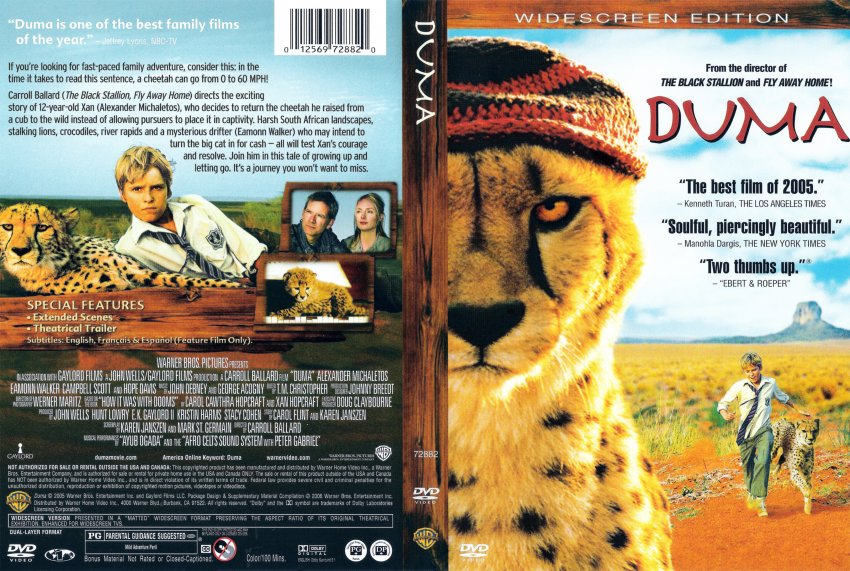
\includegraphics[width=\textwidth]{content/assets/duma--2}
  \end{center}
\end{figure}

\textit{Duma} is cheap and easy to find. I bought my copy from Amazon for £3.

This is the third of four articles on the films of Carroll Ballard. All four movies are great. Choose your species and join us:

\textit{The Black Stallion} (horse)
\textit{Never Cry Wolf} (wolf): coming soon
\textit{Fly Away Home} (goose)
\textit{Duma} (cheetah)
